\section{Optimization}
In this section we select which parameters are going to be used when building our robot.

\subsection{Minimum section in the section of the flywheel}
We wil place our flywheel in a hole on our robot. We will now compute the minimum section in hole so it doesn't bend. See figure \ref{fig:Flywheel hole diagram}.

\begin{figure}[ht]
	\centering
	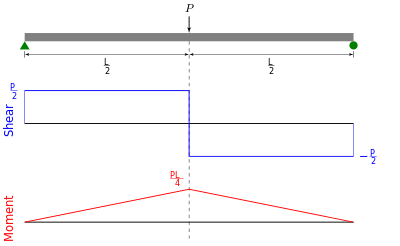
\includegraphics[width=10cm]{img/Shear_Moment_Diagram.png}
	\caption{Bendig moment diagram}
	\label{fig:Bendig moment diagram}
\end{figure}
The maximum bending moment is at the flywheel section:
\[M_y = \frac{P * L}{4}\]
Where P is the weight of the robot and L is the distance between the two wheels.

\[I_y = \frac{2*b*h^3}{12}=\frac{b*h^3}{6}\]
\[\sigma=\frac{M_y}{I_y}*\frac{h}{2} = \frac{P*L}{48*b*h^2}\]
We are planning to build our body structure with plastic:
\[\sigma_{plastic} = 4MPa = 4E6Pa\]
We will impose the relation:
\[b = h\]
And set a target P of $2000N$ and a maximum length of $0.5m$
\[\sigma_{plastic} = 4E6Pa = \frac{P*L}{48*b*h^2} = \frac{1000}{48*b^3} \]
Therefore:
\[b = \sqrt[3]{\frac{1000}{48*4E6}} = 1,277182 m\]
We will use b=10mm and h=10mm from now on. Which is far more than what we need.


\subsection{Restrictions}
The first restrictions is due to the initial design requirements. The other three are somehow arbitrary but will help us to reduce the size of the robot.
\begin{enumerate}
\item We wil place our flywheel in a hole on our robot. We don't want to touch the ground in any configuration so:
\begin{figure}[ht]
	\centering
	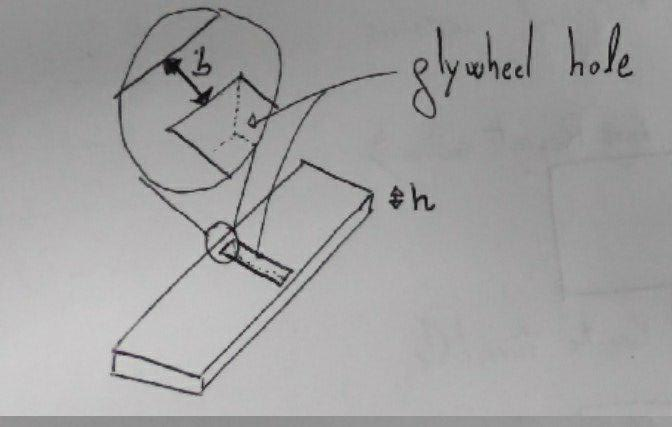
\includegraphics[width=5cm]{img/flywheel_hole.jpg}
	\caption{Flywheel hole diagram}
	\label{fig:Flywheel hole diagram}
\end{figure}
\[r_{wheel}> \sqrt{(r_{flywheel} + b)^2+(\frac{h}{2})^2}\]
\item Being able  to insert the robot in to a wheel of diameter 0.5m so:
\begin{figure}[ht]
	\centering
	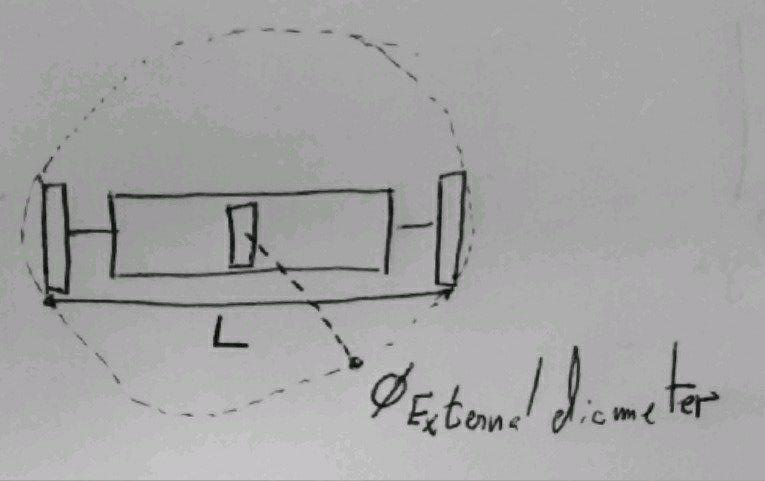
\includegraphics[width=5cm]{img/external_diameter.jpg}
	\caption{External diameter diagram}
	\label{fig:External diameter diagram}
\end{figure}
\[0.25 m > \sqrt{r_{wheel}^2 + L^2/4}\]
\item We can place all electronic the devices:
\[L > 0.3m + w \]
\item Maximum weight of the robot: 5kg
\end{enumerate}

\subsection{Requirements}
Based on the mechanical analysis we have set some requirements that we would like our robot to fullfil:
\textbf{Flywheel mode}
\begin{enumerate}
	\item $\dot{y}_{max}$ (equation \ref{Maximum speed flywheel}) $> 0.1m/s$
	\item $\ddot{y}_{max}$ (equation \ref{maximum acceleration flywheel})> $1m/s^2$
	\item $sin(\alpha_{max})$ (equation \ref{Maximum angle using flywheel system}) $> 0.2$
\end{enumerate}
\textbf{Pendulum mode}
\begin{enumerate}
	\item $\dot{y}_{max}$ (equation \ref{maximum speed pendulum}) $> 1m/s$
	\item $\ddot{y}_{max}$ (equation \ref{maximum acceleration pendulum}) $>0.1m/s^2$
	\item $sin(\alpha_{max})$ (equation \ref{Maximum angle using pendulum system}) $> 0.02$
\end{enumerate}
	


\subsection{Cost function}
Apparat from fulfilling the requirements we will try to minimize a cost function.

We will maximize the maximum sinus in the pendulum mode 
(equation \ref{Maximum angle using pendulum system}) because
it give the robot the capacity to deliver force in a permanent state.

We will also maximize the square of the max speed the robot can achieve
in flywheel mode (equation \ref{Maximum speed flywheel}) because it is
proportional to the energy the robot can deliver using the flywheel at a certain moment.

\begin{equation}
	cost(r_{flywheel},r_{wheel},w,N) = - sin(\alpha_{max})_{pendulum} -\dot{y}^2_{max-flywheel}
	\label{eq: cost}
\end{equation}
\begin{equation*}
	m_{cylinder} = \rho * w * \pi * (\frac{r_{flywheel}}{3})^2
\end{equation*}
\begin{equation*}
	sin(\alpha_{max})_{pendulum} = \frac{m_{cylinder} \cdot  (r_{max} - r_{min})}{m_{total} \cdot r_{wheel}} = \frac{m_{cylinder} \cdot  (\frac{r_{flywheel}}{3})}{(m_{rest} + N \cdot m_{cylinder})\cdot r_{wheel}} 	
\end{equation*}
\begin{equation*}
	\dot{y}_{max} = r_{wheel} \cdot  R \cdot  \dot{\theta}_{max} =r_{wheel} \cdot  \frac{ N \cdot  m_{cylinder} \cdot  (\frac{2\cdot r_{flywheel}}{3})^2}
    {r_{wheel}^2\cdot (m_{rest} + N \cdot m_{cylinder}) +  2\cdot I_{wheel}} \cdot  \dot{\theta}_{max}
\end{equation*}

\subsection{Results}
Our procedure has been making a grid with the four parameters of the robot 
design: $w$ (width of the cylinders), $N$(number of cylinders), $r_{wheel}$ and $r_{flywheel}$.
We have fixed $r_{flywheel}$, iterated over the other three variables and keeped the best parameters to reduce our cost function.


\begin{figure}[H]
	\centering
	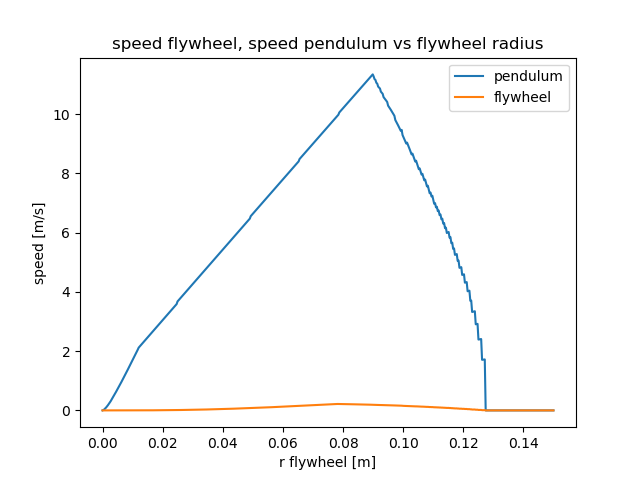
\includegraphics[width=10cm]{img/optimization/speed.png}
	\caption{Plot of the equations \ref{Maximum speed flywheel} and \ref{maximum speed pendulum} at the parameters that minimize the cost function and fullfil the requirements and restrictions}
	\label{fig:Speed plot}
\end{figure}

\begin{figure}[H]
	\centering
	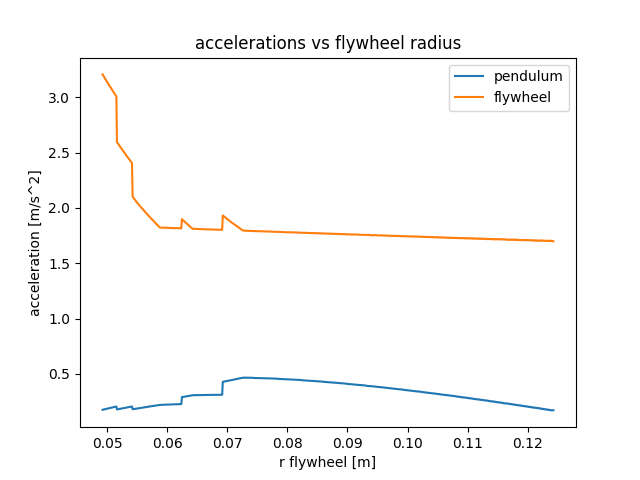
\includegraphics[width=10cm]{img/optimization/acceleration.png}
	\caption{Plot of the equations \ref{maximum acceleration flywheel} and \ref{maximum acceleration pendulum} at the parameters that minimize the cost and fullfil the requirements and restrictions}
	\label{fig:Speed plot}
\end{figure}

\begin{figure}[H]
	\centering
	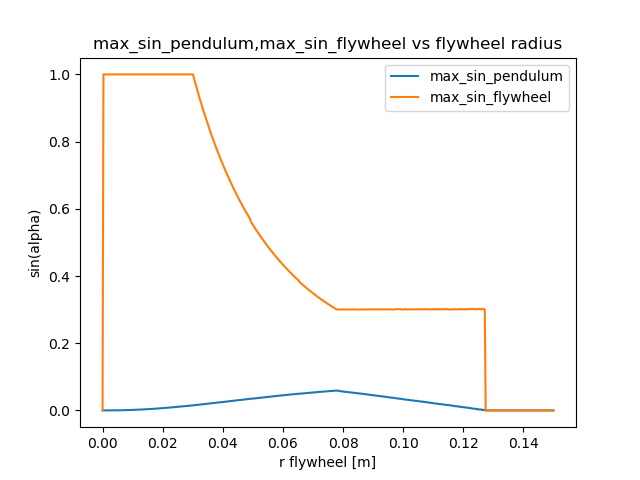
\includegraphics[width=10cm]{img/optimization/sin.png}
	\caption{Plot of the equations \ref{Maximum angle using flywheel system} and \ref{Maximum angle using pendulum system} at the parameters that minimize the cost and fullfil the requirements and restrictions}
	\label{fig:Sinus plot}
\end{figure}

\begin{figure}[H]
	\centering
	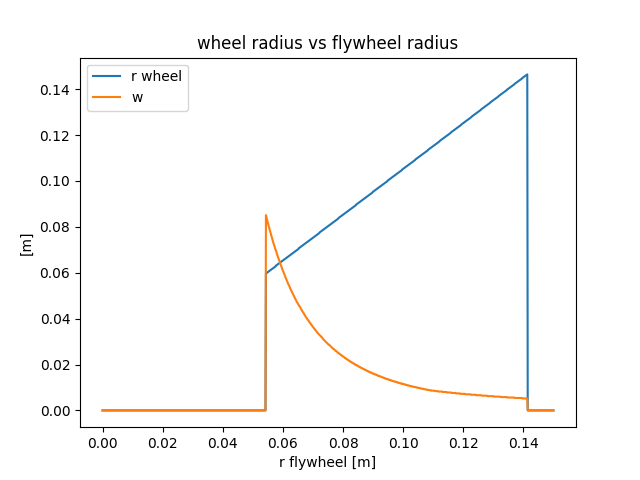
\includegraphics[width=10cm]{img/optimization/parameters.png}
	\caption{Plot of the parameters that minimize the cost function.}
	\label{fig:Parameters plot}
\end{figure}

\begin{figure}[H]
	\centering
	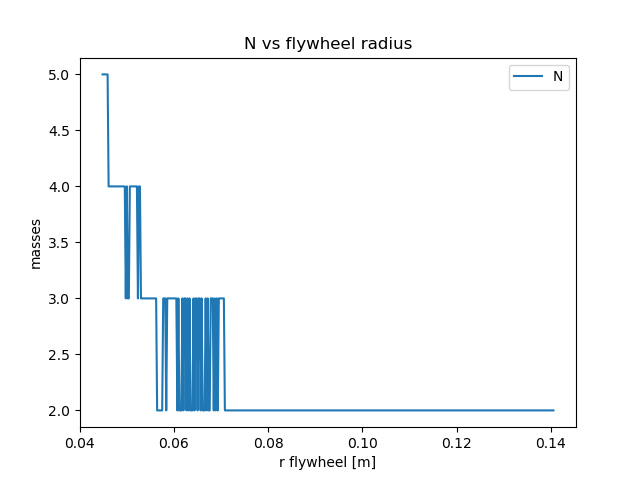
\includegraphics[width=10cm]{img/optimization/N.png}
	\caption{Plot of the N that minimize the cost function.}
	\label{fig:Parameters plot}
\end{figure}

\begin{figure}[H]
	\centering
	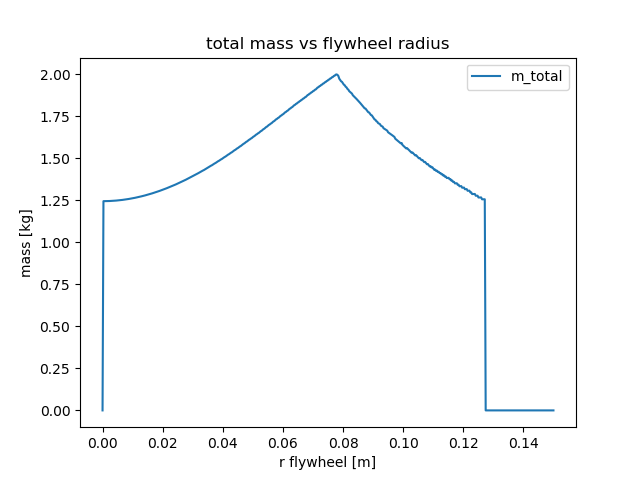
\includegraphics[width=10cm]{img/optimization/mass.png}
	\caption{Plot of the mass for each configuration.}
	\label{fig:Mass plot}
\end{figure}

%\begin{figure}[H]
%	\centering
%	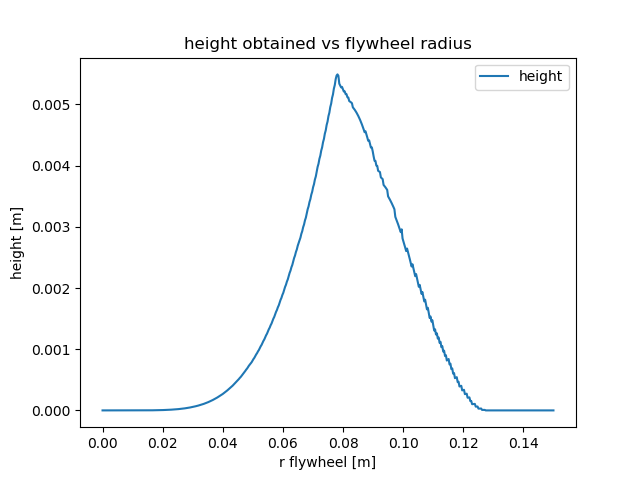
\includegraphics[width=10cm]{img/optimization/height.png}
%	\caption{Plot of the equation \ref{Maximum height} for each configuration.}
%	\label{fig:Mass plot}
%\end{figure}

\begin{figure}[H]
	\centering
	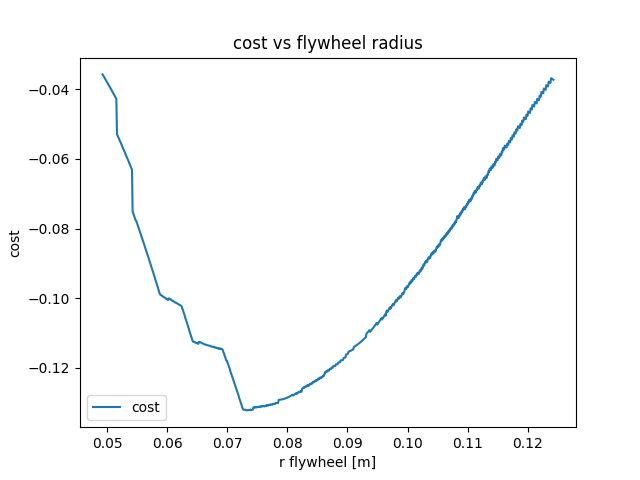
\includegraphics[width=10cm]{img/optimization/cost.png}
	\caption{Plot of the equation \ref{eq: cost} for each configuration.}
	\label{fig:Mass plot}
\end{figure}

Our selected parameters are:
\begin{center}
	\begin{tabular}{ |c|c|c|c| } 
	 \hline
	 $r_{flywheel}$ & $r_{wheel}$ & $w$ & $N$\\
	 \hline 
	 8cm & 10cm & 5cm & 2 \\ 
	 \hline
	\end{tabular}
\end{center}

With this parameters we get the following specifications:
\begin{center}
	\begin{tabular}{ |c|c| } 
	 \hline
	 Total mass & 2,91kg\\
	 \hline
	 \textbf{Pendulum} \\
	 \hline
	 Maximum sinus & 0,042\\
	 \hline
	 Maximum speed horizontal & 1,84 $m/s$\\
	 \hline
	 Maximum acceleration horizontal & 0,38 $m/s^2$\\
	 \hline
	 \textbf{Flywheel} \\
	 \hline
	 Maximum sinus & 0,171\\
	 \hline
	 Maximum speed horizontal & 0,24 $m/s$\\
	 \hline
	 Maximum acceleration horizontal & 1.52 $m/s^2$\\
	 \hline
	\end{tabular}
\end{center}